\documentclass[tikz,fontsize=8pt]{standalone}
\usepackage{scrextend}
\usepackage{fourier}
\usetikzlibrary{arrows.meta}
\usetikzlibrary{calc}
\tikzset{>=latex}
\definecolor{bookblue}{RGB}{0,173,239}
\definecolor{bookpink}{RGB}{236,0,140}
\definecolor{bookgreen}{RGB}{50,200,0}
\definecolor{bookbluearea}{RGB}{204,239,252}
\tikzstyle{blueline}=[draw=bookblue,line width=0.2mm]
\tikzstyle{pinkline}=[draw=bookpink,line width=0.2mm]
\tikzstyle{greenline}=[draw=bookgreen,line width=0.2mm]
\tikzstyle{blackline}=[draw=black,line width=0.2mm]
\tikzstyle{bluearea}=[fill=bookbluearea]

\usetikzlibrary{quotes,arrows.meta}
\changefontsizes[8pt]{8pt}
\usetikzlibrary{decorations.pathreplacing}
\usepackage[utf8]{inputenc}
\begin{document}
  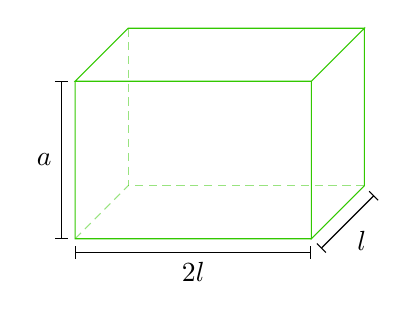
\begin{tikzpicture}[every edge quotes/.append style={auto, text=black}]
  \pgfmathsetmacro{\cubex}{3}
  \pgfmathsetmacro{\cubey}{2}
  \pgfmathsetmacro{\cubez}{1.75}
  \draw [draw=bookgreen, every edge/.append style={draw=bookgreen, densely dashed, opacity=.5}, fill=none]
  (0,0,0) coordinate (o) -- ++(-\cubex,0,0) coordinate (a) -- ++(0,-\cubey,0) coordinate (b) edge coordinate [pos=1] (g) ++(0,0,-\cubez)  -- ++(\cubex,0,0) coordinate (c) -- cycle
  (o) -- ++(0,0,-\cubez) coordinate (d) -- ++(0,-\cubey,0) coordinate (e) edge (g) -- (c) -- cycle
  (o) -- (a) -- ++(0,0,-\cubez) coordinate (f) edge (g) -- (d) -- cycle;
  \path [every edge/.append style={draw=black, |-|}]
  (b) +(0,-5pt) coordinate (b1) edge ["$2l$"'] (b1 -| c)
  (b) +(-5pt,0) coordinate (b2) edge ["$a$"] (b2 |- a)
  (c) +(3.5pt,-3.5pt) coordinate (c2) edge ["$l$"'] ([xshift=3.5pt,yshift=-3.5pt]e)
  ;
  \end{tikzpicture}
\end{document}